\chapter{MEG source localisation\label{Chap:data:sloc}}


\section{Overview}
In this section we will generate some simulated data to show how the inversion algorithms compare when the ground-truth is known. 

\section{Simulation}
The easiest way to simulate M/EEG data is by replacing data from an existing experimental recording in which sensor locations/head position etc are already defined. You can do this using the batch editor. Start the batch editor (\texttt{Batch} button) on main panel. Then from the dropdown menu SPM: select \texttt{M/EEG}; select \texttt{Source reconstruction}; select \texttt{Simulation of sources on cortex}.
You will see the following menu:

\begin{figure}
\begin{center}
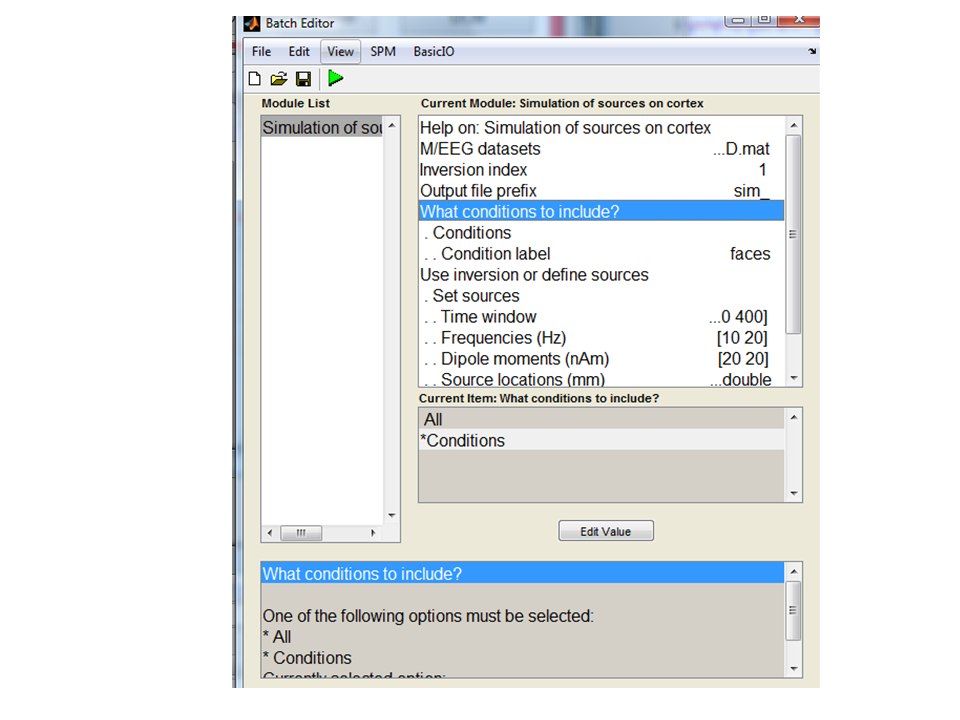
\includegraphics[width=100mm]{meg_sloc/slide1}
\caption{\em The simulation batch options} \label{meg_sloc:fig:1}
\end{center}
\end{figure}

You can use any SPM file you like to provide the basic simulation set up: this file will include information on sensor locations, triggers, head model. As an example we can use the preprocessed multimodal face-evoked MEG dataset\footnote{Multimodal face-evoked dataset: \url{http://www.fil.ion.ucl.ac.uk/spm/data/mmfaces/}}. So for M/EEG dataset select 

\begin{verbatim}
cdbespm12_SPM_CTF_MEG_example_faces1_3D.mat
\end{verbatim}

\texttt{Inversion index} allows you to determine which forward model/ inversion is used to simulate data, leave this at the default value (1) for now.
\texttt{Output file prefix} allows you to specify the prefix to be added to the new file.
Under 'what conditions to include',  you can either specify to simulate data in all experimental conditions 'All' or in specific conditions only. Here we want to test between conditions so we will simulate data  in only one condition. Select the \texttt{Conditions} option and for \texttt{Condition labe}'  type 
\begin{verbatim}
faces
\end{verbatim}

The next option \texttt{Use inversion or define sources} allows you to either re-generate data based on a previous source reconstruction (and vary the SNR) or to set up a number of active sources on the cortical surface. We will use the last option, select \texttt{Set sources}. You can use the default options for now which defines two sources at different frequencies in approximately the auditory cortices.

That is, the two dipoles are currently set to be on (at 10 and 20Hz) during the faces condition and off during the scrambled condition.

This file has dipoles at [52, -25, 9] and  [-52, -25, 9] in MNI space. The dipoles are energized at 10Hz and 20Hz from 0.1 to 0.4 seconds (Figure~\ref{meg_sloc:fig:1}). In each epoch the activation profile is identical, the channel data will be slightly different due to the white noise added. The green arrow in the top left menu bar should light up when all the essential parameters have been input and you can press it to run the simulation.

\begin{figure}
\begin{center}
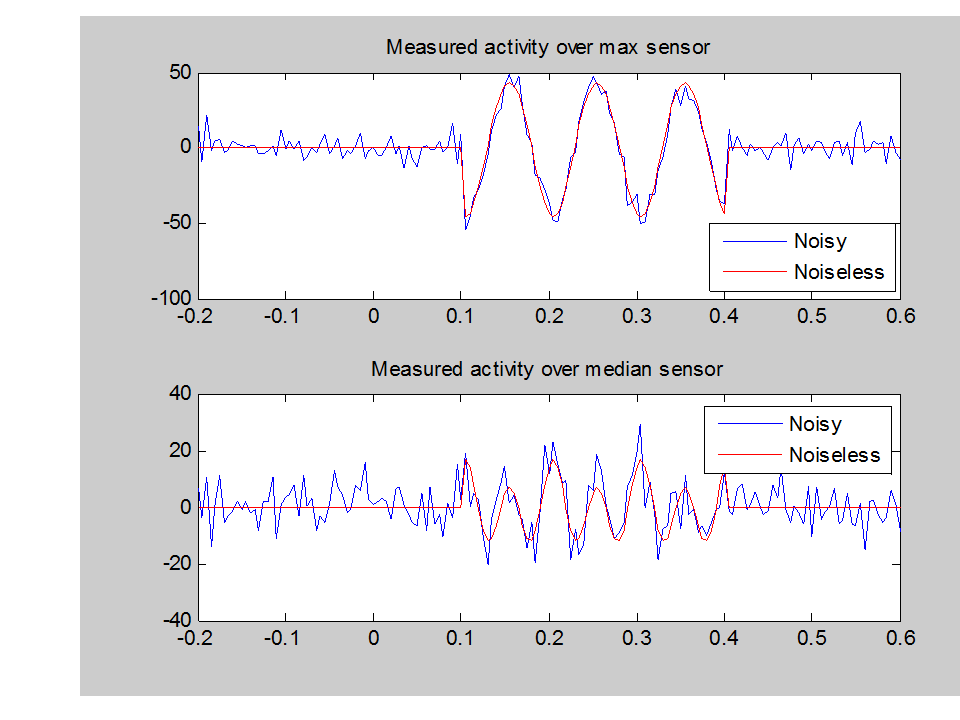
\includegraphics[width=100mm]{meg_sloc/slide2}
\caption{\em The simulation outputs a glass brain showing maximum and median channel time-series as well as a glass brain showing the locations at which the sources were simulated } \label{meg_sloc:fig:2}
\end{center}
\end{figure}

You can visualise the data trial by trial if you like by using the main menu Display/MEEG button.
\section{Imaging solutions for evoked or induced responses}

There are two pathways you can take to analyse the data. Either with the GUI buttons or with the batch interface. 

Firstly lets use the GUI to check that the data is ready for source inversion. On the main menu Click \texttt{3D Source Reconstruction}. Press \texttt{Load}. Select the new simulated data file \texttt{sim\_cdbespm12\_SPM\_CTF\_MEG\_example\_faces1\_3D.mat}.

Moving left to right along the bottom panel you will notice that all of the buttons (MRI, Co-register, Forward Model) are active. This means that the preprocessing stages have already been carried out on these data (see multi-modal evoked responses chapter).

 The advantage of the batch interface is that you can then build up large and automated analysis pathways, it also is a little more flexible so it has more functionality.

So restart the Batch editor from the main menu \texttt{Batch}. Then from the \texttt{SPM} drop-down menu select \texttt{M/EEG} / \texttt{source reconstruction} / \texttt{Source inversion}.

Select the new simulated data file \texttt{sim\_cdbespm12\_SPM\_CTF\_MEG\_example\_faces1\_3D.mat}.
Now we wish to invert all conditions using the same assumptions (and then compare between conditions afterwards) so under 'what conditions to include' select 'All'.
At this point we can now try out inversion algorithms with different implicit assumptions. Under \texttt{Inversion parameters} select \texttt{Custom}.
We will modify \texttt{inversion type} in the subsequent sections. Select \texttt{IID} for minimum norm assumptions for now.
For the \texttt{Time window of interest} select from 0 to 600ms. For the \texttt{frequency window of interest} select 0 to 80 Hz  (our data were simulated at 10 and 20Hz between 100 and 400ms).
All the other settngs should remain as default.

\begin{figure}
\begin{center}
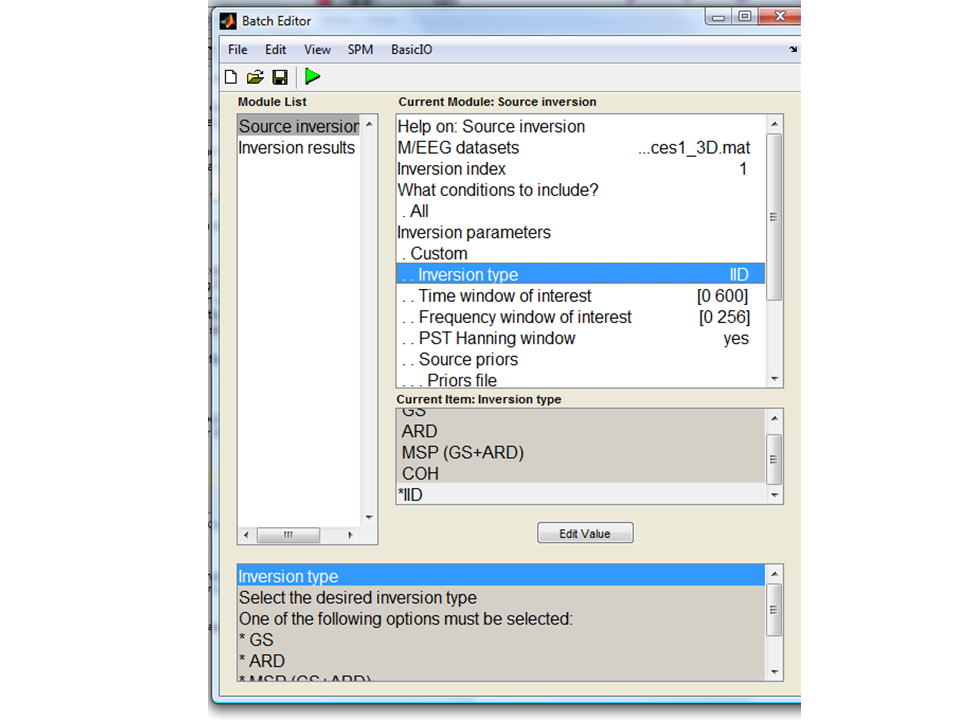
\includegraphics[width=100mm]{meg_sloc/slide3}
\caption{\em The basic batch settings for the source inversion} \label{meg_sloc:fig:3}
\end{center}
\end{figure}

\subsection{IID (minimum norm)}
We will start off with the traditional minimum norm solution: the 'IID' inversion type option . This starts by assuming that all source elements contribute something to the measured data. The constraint is that the total power (in the sources) should be minimised.
Press \texttt{Invert}. Under reconstruction method press \texttt{Imaging}. For \texttt{All conditions or trials} press \texttt{Yes}. For model press \texttt{Custom}. Model inversion \texttt{IID}. Under Time-window ``0 600''. For \texttt{PST Hanning} select \texttt{Yes}. For High-pass (Hz) select \texttt{1} for Low-pass (Hz) select \texttt{48}. For \texttt{Source priors}, select \texttt{No}. Under \texttt{Restrict solutions} select \texttt{No}. 

\begin{figure}
\begin{center}
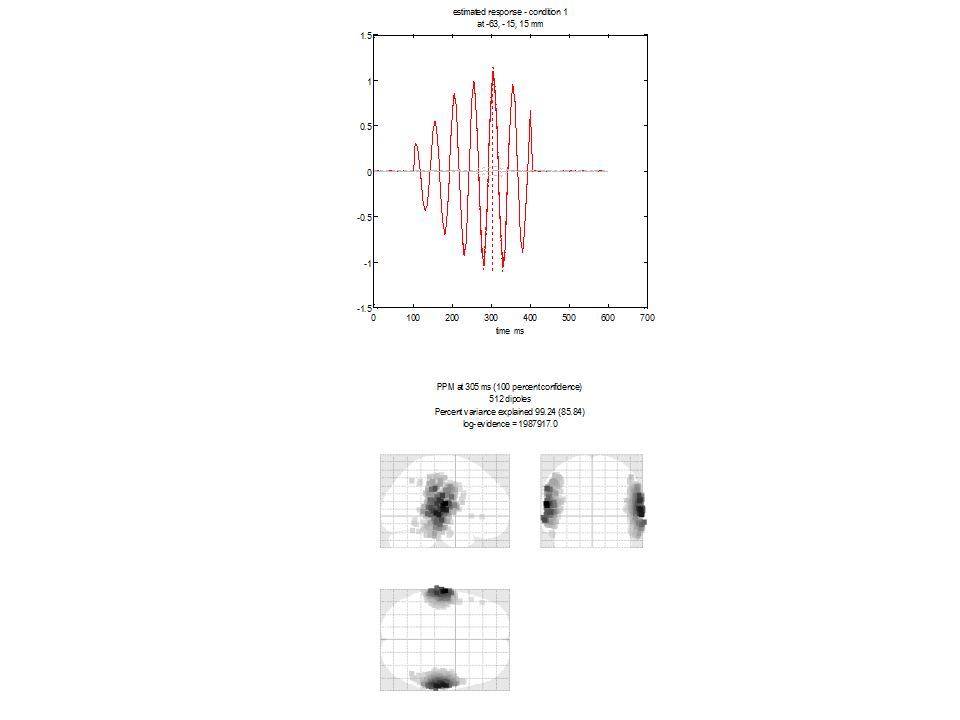
\includegraphics[width=100mm]{meg_sloc/slide4}
\caption{\em IID imaging source reconstruction \label{meg_sloc:fig:4}}
\end{center}
\end{figure}

 
We see the anticipated minimum norm result. The current density estimate is diffuse and relatively superficial due to the minimum energy constraint.  Note the log-evidence 1987917 (this value depends on the data - so value of the log evidence you see may be different but it is this value relative to those following which is important).
The top panel shows two time-series extracted from the mesh vertex (location given at the top of the panel) with highest posterior probability.  The red line corresponds to the first condition (faces). Note the sinsuoidal time-series which should correspond in frequency to the source simulated on that side of the brain. The grey line corresponds to the other condition (scrambled) in which no data were simulated.


\subsection{Smooth priors (COH)}
The \texttt{COH}, under \texttt{Inversion type}, option allows the mixture of two possible source covariance matrices: the minimum norm prior above and a much smoother source covariance matrix in which adjacent sources are correlated (over the scale of a few mm). Select \texttt{COH} as the custom source reconstruction and run the batch again.
 
 You will see a plot similar to Figure~\ref{meg_sloc:fig:5} appear. The lower panel shows the glass brain in which bilateral sources are apparent. The upper panel shows the time-series of the source with the largest amplitude. In this case the peak activation is identified at location 59,-15, 15mm. The 20Hz time-course (associated with this source) is also clearly visible in the top panel.  Log evidence is 2000393  (again this number may be different in your spm version). Note both that the source reconstruction is more compact and that the log evidence has increased over the IID solution.

\begin{figure}
\begin{center}
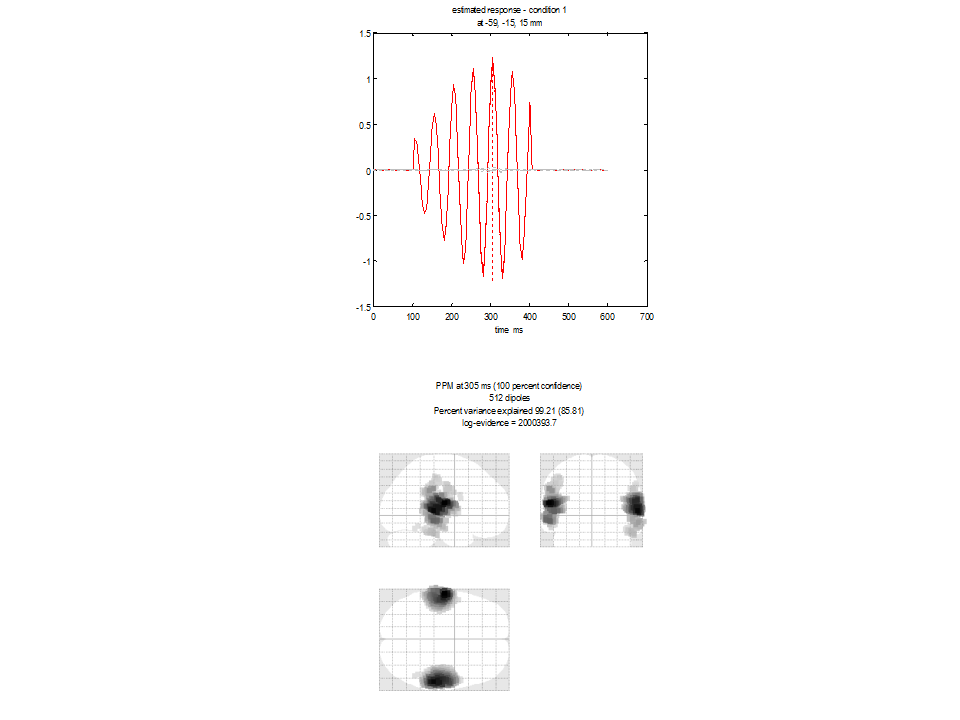
\includegraphics[width=100mm]{meg_sloc/slide5}
\caption{\em COH imaging source reconstruction.\label{meg_sloc:fig:5}}
\end{center}
\end{figure}



\subsection{The Multiple sparse priors algorithm}

\begin{figure}
\begin{center}
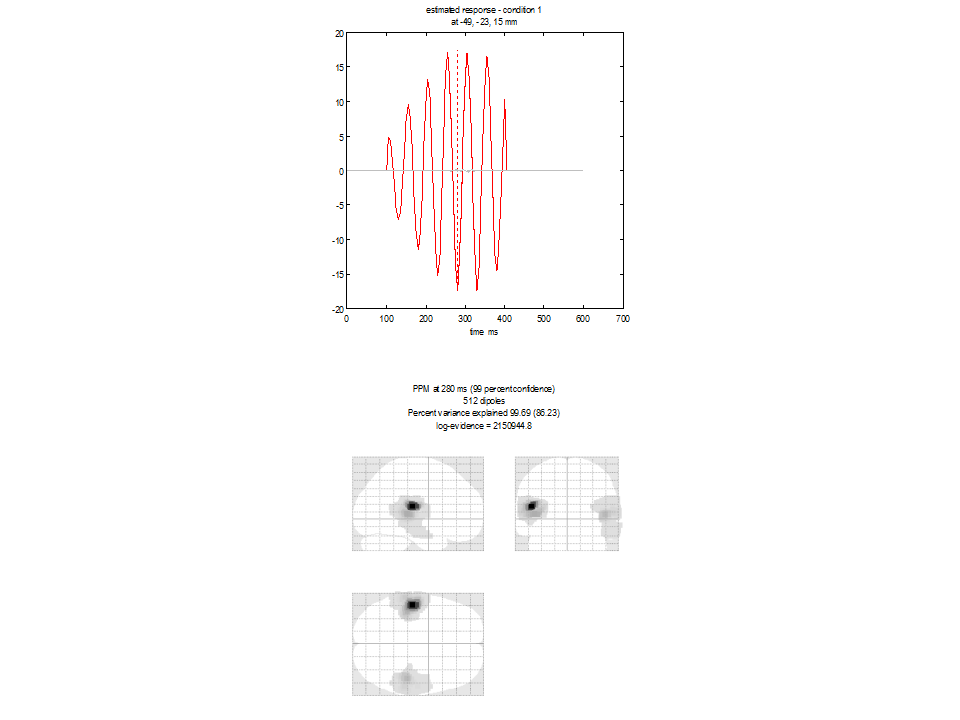
\includegraphics[width=100mm]{meg_sloc/slide6}
\caption{\em Multiple sparse priors imaging source reconstruction using the Greedy Search (GS) option.\label{meg_sloc:fig:6}}
\end{center}
\end{figure}

In contrast to IID or COH, the greedy search routine used in MSP builds up successive combinations of source configurations until the model evidence can no longer be improved. 
Select \texttt{GS} as the inversion type and run the batch again. You will see a plot similar to Figure~\ref{meg_sloc:fig:6} appear. The lower panel shows the glass brain in which bilateral sources are apparent. The upper panel shows the time-series of the source with the largest amplitude.  Again the source reconstruction is compact with log evidence is 2150944. Note both that the source reconstruction is more compact and that the log evidence has increased over the IID and COH solutions.
There are two more options in the basic MSP implementaion- ARD- based on the removal of patches that contribute little to the model evidence; and the use of both schemes 'ARD and GS' in which both methods provide candidate source covariance estimates which are then combined.  You can try out these other options for yourself and note the model evidences (which will be directly comparable as long as the data do not change).

\subsection{Making summary images}
Often we will interested in some summary of conditions over a specific time-frequency window. We can add in an extra module to the batch script to produce such an output. .

From the \texttt{SPM} drop down menu click \texttt{M/EEG}/  \texttt{Source reconstruction}/  \texttt{Inversion results}. Now for \texttt{M/EEG dataset}, click \texttt{Dependency}- and press OK to link the output of the previous function (the inversion) to the inpput of this one. We can now produce power images per condition based on a 0 to 600ms time window and a 0 to 80Hz frequency window. For \texttt{Contrast type} select \texttt{Evoked} and for output space and format select \texttt{MNI} and  \texttt{Mesh} .

You should now be able to run the complete batch which re-does the inversion and outputs two surface meshes (one for each condition). You can view these meshes from the main menu : \texttt{Render}/ \texttt{Display}. The output image for the face condition (and the IID algorithm) is shown below. 


\begin{figure}
\begin{center}
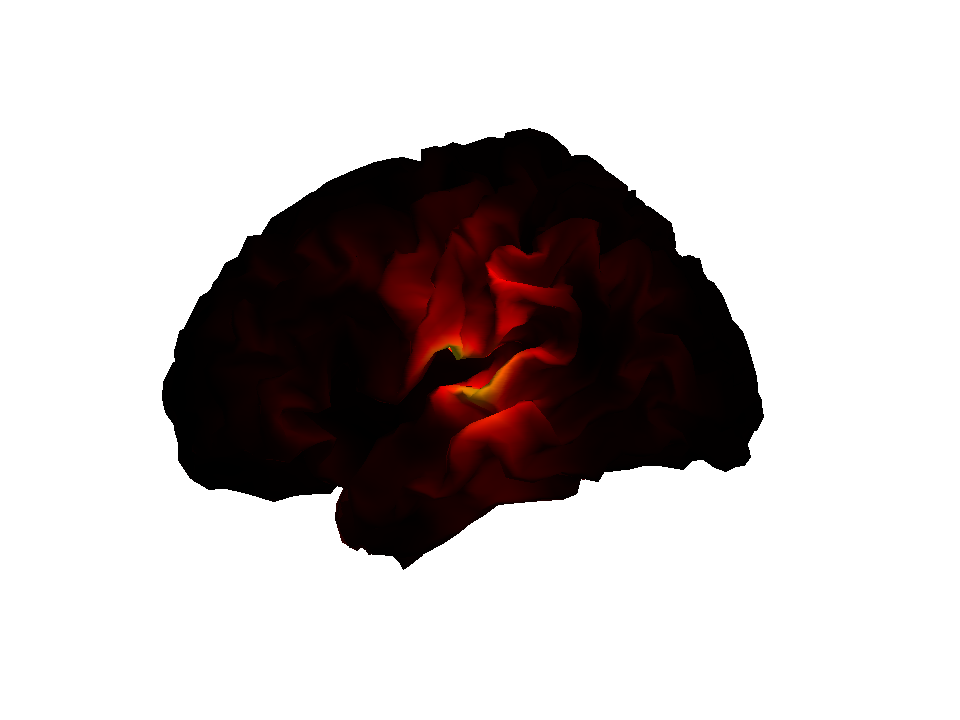
\includegraphics[width=100mm]{meg_sloc/slide7}
\caption{\em Summary power image from IID source reconstruction on mesh.\label{meg_sloc:fig:7}}
\end{center}
\end{figure}


\subsection{Other MSP options}

The MSP algorithm is optimized to give the simplest source distribution that explains the most data. However the library of priors (possible patch locations) must be pre-specified in advance. This could potentially cause a problem if the source of interest were not precisely centred on one of the patches in the default library. To this end Jose David Lopez (Conf Proc IEEE Eng Med Biol Soc. 2012;2012:1534-7.) has produced a version of MSP which uses multiple random patch libraries to invert the same data several times. 
We can make a new batch file for this. So restart the Batch editor from the main menu \texttt{Batch}. Then from the \texttt{SPM} drop-down menu select \texttt{M/EEG} /  \texttt{source reconstruction} / \texttt{Source inversion, iterative}.

Select \texttt{Classic} as the custom source reconstruction algorithm- this is basically the original version of the MSP algorithm without any re-scaling factors to allow mixing of modalies or group imaging. It is advanatageous in many cases as the lack of these scaling factors means that it is a true generative model of the data (and it becomes possible to test between different head positions etc). Note however that these differences in pre-processing mean that at the moment the data entering the inversion (for custom and classic options) are different and so it is not possible to compare between solutions from these two pipleines.
 The rest of the parameters (time, frequency windows etc) can remain as they were in the last section. The new options are the choice over the number of patches in the library  and the number of iterations. You can play with these parameters to adjust the relative burden of computation time. For example- allowing just 2 patches and many iterations will make this something like a (cortically constrained) multiple dipole (patch) fit. Alternatively, having lots of patches initially will mean the computation time is spent on pruning this set (with ARD or GS etc). 
You also have control over the number of temporal and spatial modes which will be used here (this makes it easier to compare between models where the lead field matrix has changed). 
The alogorithm returns the current distribution based on the patch set with maxmum free energy.

\begin{figure}
\begin{center}
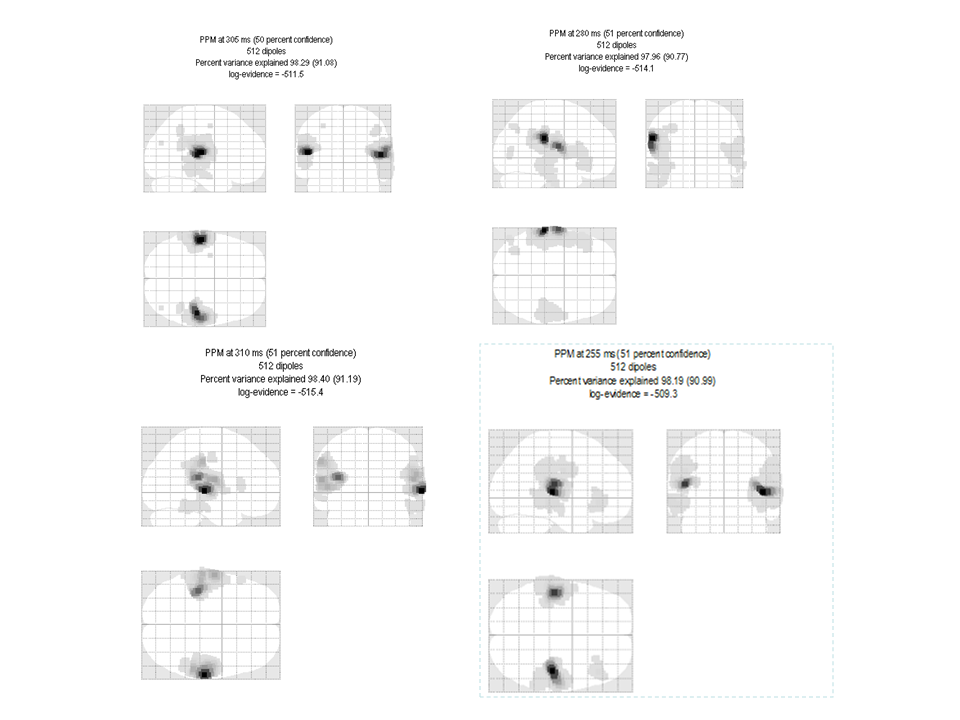
\includegraphics[width=100mm]{meg_sloc/slide8}
\caption{\em  Source inversions based on the same data but using randomly selected sets of 512 spatial priors.\label{meg_sloc:fig:8}}
\end{center}
\end{figure}


An alternative to many spatial priors is to have a single prior that is optimised using functional constraints. This idea was put forward by Belardinelli P et al. PLoS One. 2012;7(12). Here a single candidate source covariance is estimated using beamformer priors and then regularized (in much the same way as IID and COH matrices are) in the Bayesian framework. You can access this by selecting \texttt{EBB} (Empirical Bayes Beamformer) as the inversion type; but you should set the number of iterations here to 1 (as there is only a single prior and it will not change over repetiitions).

\begin{figure}
\begin{center}
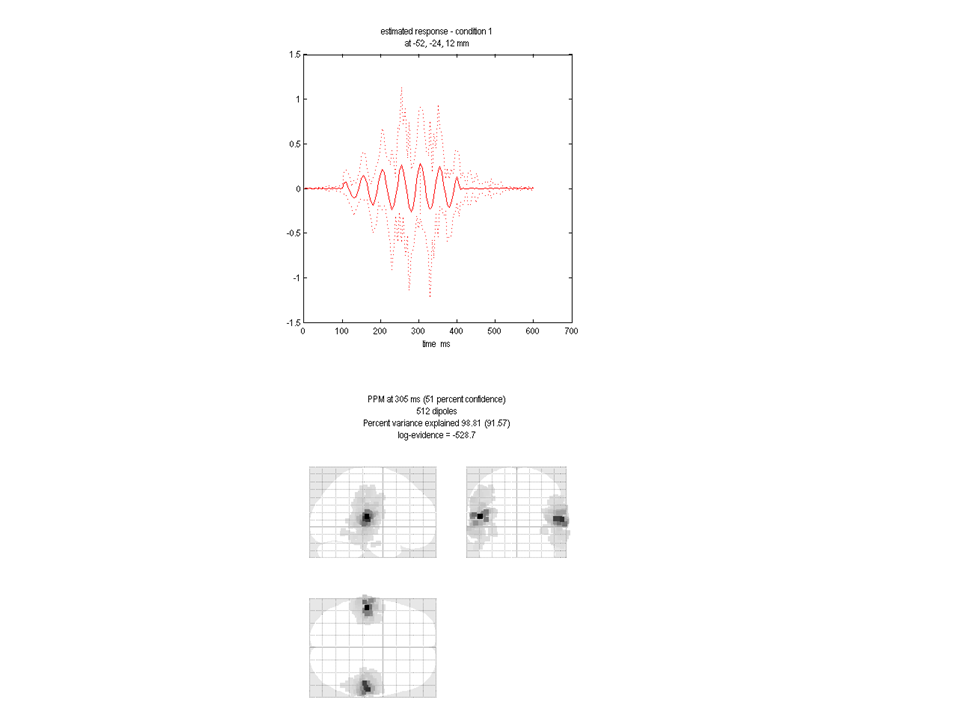
\includegraphics[width=100mm]{meg_sloc/slide9}
\caption{\em  Source inversions based on the same data but using a single beamformer prior.\label{meg_sloc:fig:9}}
\end{center}
\end{figure}

You can see that the beamformer image is much more focal than any other image type (and it is fast to compute). However there will be many situations in which it is sub-optimal (such as if you were to simulate two correlated sources). In Belardinelli et al. the authors found that this failure was reflected in the free energy; meaning that it is still possible to directly compare this solution with GS , IID etc.



\section{Dipole fitting to the average}

 Up until this point the analysis we have used could have been applied to either induced or evoked changes in electrical activity. The only difference being that it would not have made much sense to look at the MSPs for specific time-instants in the induced case and we would have proceeded directly to look for changes in a time-frequency window. To examine the dipole fit routine we will however concentrate on the averaged data file which will contain only evoked changes. 
For this final section we will revert back to the main gui.
Press  \texttt{Average}. Select the simulated data file and leave all of the other options as default.

Press  \texttt{3D source Reconstruction}.

\subsection{Load/preview the data}

In the main menu click on the drop-down \texttt{Display} menu. Select \texttt{M/EEG}. For the dipole fitting we are going to use averaged MEG data, this is prefixed with an ``m'' in SPM. You can generate this file by averaging the epoched file that we have used until now. Select the file \texttt{msim\_cdbespm12\_SPM\_CTF\_MEG\_example\_faces1\_3D.mat}.

The two sources we simulated were at 10Hz an 20Hz frequency so we can select times when only one or both of them were active.  At 235ms there is only one dominant source and at 205ms both sources are clearly visible at the sensor level.

We will now move on to explore Bayesian dipole fitting to these two time instants.

\subsection{Inversion}
In the main menu window, select \texttt{3D Source Reconstruction}. Click \texttt{Load} and select the averaged simulated dataset above.
Proceed by pressing the \texttt{Invert} button. Select the \texttt{VB-ECD} button.

\subsubsection{Fitting a single dipole with no priors}
At the \texttt{time\_bin or average\_win} prompt enter ``235''. For \texttt{Trial type number} choose ``1'' (we want to model the faces data). At the \texttt{Add dipoles to model} click \texttt{Single}. For \texttt{location prior} click \texttt{Non-info}. For \texttt{Moment prior} click \texttt{Non-info}. At the \texttt{Add dipoles to 1 or stop?} prompt click \texttt{stop}. At the \texttt{Data SNR (amp)} leave as default \texttt{5}. Leave the default number of iterations at ``10''.
You will see the 10 successive fits of the same data using a random starting location and moment. At each fit maps of the predicted and simulated data along with free-energy values and percent variance explained are shown. The final plot will be similar to Figure~\ref{meg_sloc:fig:10} where the model (i.e. dipole) which maximised the evidence (the best iteration is shown with a red dot) is displayed. Note down the model evidence (in this case -7.508e2, but the absolute value in your implementation may be different). The Bayesian dipole fit algorithm will be most useful when one has some prior knowledge of the sources (such as location, orientation or symmetry). Typical dipole fit algorithms fit 3 location parameters per dipole and then estimate the moment through a pseudo-inverse. The VB-ECD algorithm however fits 6 parameters per dipole as the moments are also allowed prior values. That is, if you have no prior knowledge then the Bayesian method will be generally less robust than such fitting methods (as more parameters are being fit). However it is when prior knowledge is supplied that the Bayesian methods become optimal.

\begin{figure}
\begin{center}
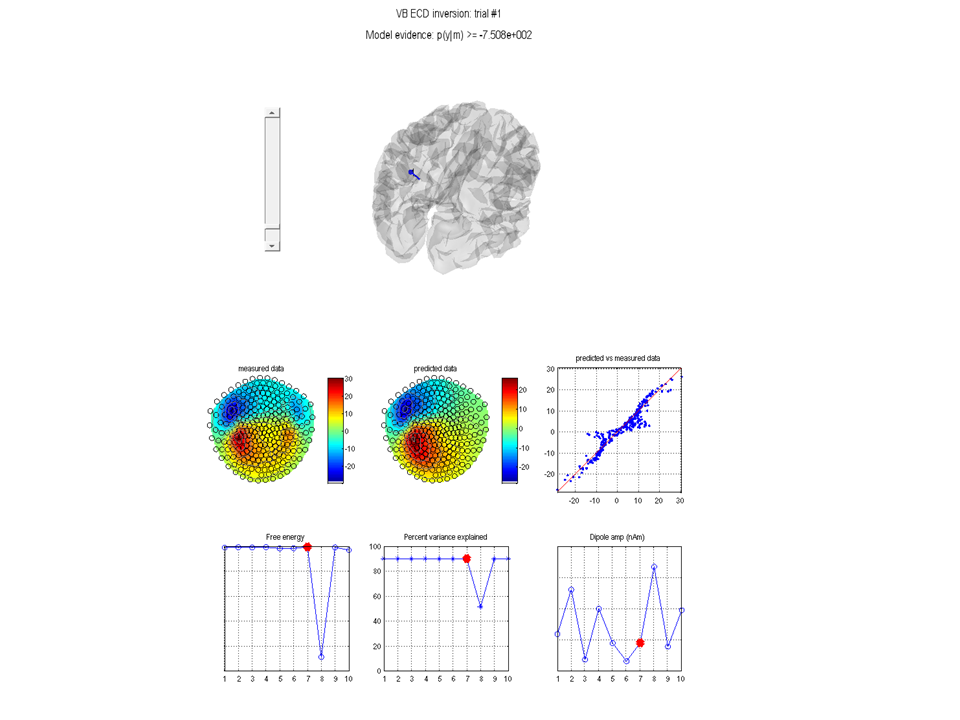
\includegraphics[width=140mm]{meg_sloc/slide10}
\caption{\em Results of fitting a single dipole with noninformative priors.\label{meg_sloc:fig:10}}
\end{center}
\end{figure}


\subsubsection{Fitting a single dipole with reasonable and unreasonable priors}
We will now provide some prior knowledge to the dipole fit perhaps led by the literature or a particular hypothesis. In this case we know the answer, but let us specify a location a couple of cm from where we know the source to be and try the fit again.
At the  \texttt{time\_bin or average\_win} prompt enter ``235''. For  \texttt{Trial type number} choose ``1'' (we want to model the faces data). At the  \texttt{Add dipoles to model} click  \texttt{Single}. For  \texttt{location prior} click  \texttt{Informative}. For the location enter ``-62 -20 10''. For prior location variance leave at ``100 100 100'' mm$^2$. This means that we are not sure about the source location to better than 10mm in each dimension. For  \texttt{Moment prior} click  \texttt{Non-info}. At the  \texttt{Add dipoles to 1 or stop?} prompt click  \texttt{stop}. Leave the default number of iterations at ``10''. Again you will get a final fit location and model evidence (-7.455e2), which should have improved (be more positive) on the evidence above (because in this case our prior was more informative). 
Now go through exactly the same procedure as above but for the prior location enter ``-62 +20 10'', i.e. on the wrong side of the head. You will note that the algorithm finds the correct location but the evidence for this model (with the incorrect prior) is lower (-7.476e2).

\subsubsection{Fitting more dipoles}
We will start by examining the time instant at which we can clearly see a two-dipolar field pattern.
At the \texttt{time\_bin or average\_win} prompt enter ``205'' (not that we are now changing the data so the subsquent evidence values will not be comparable with those at 235ms). For \texttt{Trial type number} choose ``1''. At the \texttt{Add dipoles to model} click \texttt{Single}. For \texttt{location prior} click \texttt{Informative}. For the location enter ``62 -20 10''. For prior location variance enter ``400 400 400'' mm$^2$, that is, the prior standard deviation on the dipole location is 20mm in each direction. For \texttt{Moment prior} click \texttt{Non-info}. At the \texttt{Add dipoles to 1 or stop?} prompt click \texttt{Single}. For \texttt{location prior} click \texttt{Informative}. For the location enter ``-62 -20 10''. For prior location variance enter ``400 400 400'' mm$^2$. At the \texttt{Add dipoles to 1 or stop?} prompt click \texttt{stop}. Leave the default number of iterations at ``10''. Note down the final model evidence (-2.548e2). 

Alternatively we can exploit the fact that we have prior knowledge that the dipoles will be approximately left-right symmetric in location and orientation (this means we have fewer free parameters or a simpler model). At the \texttt{time\_bin or average\_win} prompt enter ``205''.  For \texttt{Trial type number} choose ``1''. At the \texttt{Add dipoles to model} click \texttt{Symmetric Pair}. For \texttt{location prior} click \texttt{Informative}. For the205 location enter \texttt{62 -20 10}. For prior location variance enter ``400 400 400'' mm$^2$. For \texttt{Moment prior} click \texttt{Non-info}. At the \texttt{Add dipoles to 2 or stop?} prompt click \texttt{stop}.  Leave the default number of iterations at ``10''. Note that the final locations are approximately correct, but importantly the model evidence (-5.235e2) is lower than previously. Given this information one would accept the (more complex) two distinct dipole model over the symmetric pair model.


